\documentclass[12pt]{article} 

\usepackage[a4paper,
            bindingoffset=0.2in,
            left=0.75in,
            right=0.52in,
            top=0.75in,
            bottom=1.44in,
            footskip=.25in]{geometry}

\usepackage{graphicx}
\graphicspath{ {./image/} }

\usepackage{array}
{\renewcommand{\arraystretch}{2}% for the vertical padding

\usepackage{parskip}
\setlength{\parindent}{0pt}

\setcounter{secnumdepth}{0}

\title{Epidemic Modelling SIR Model}
\author{Amrit Baral, , Nabin Da Shrestha, Nirajan Bekoju, Nishant Luitel}
\date{August 23, 2022} 

\begin{document}  

\bigskip
\bigskip
\bigskip
\bigskip

\begin{center}
\includegraphics[scale = 0.5]{logo.png}

Tribhuwan University

Institute of Engineering

Pulchowk Campus

\bigskip
\bigskip
\bigskip
\bigskip

\noindent\makebox[\linewidth]
{\rule{15cm}{0.4pt}}
A Project Report on:

\textbf{\large Gravity Simulation}
\noindent\makebox[\linewidth]
{\rule{15cm}{0.4pt}}

\bigskip
\bigskip
\bigskip
\bigskip
\textbf{Submitted By:}

Amrit Baral(076bct006)

Nabin Da Shrestha(076bct037)

Nirajan Bekoju(076bct039)

Nishant Luitel (076bct041)

\bigskip
\bigskip
\bigskip
\bigskip
\textbf{Submitted To:}

Department of Electronics and Computer Engineering

\bigskip
\bigskip
\bigskip
\bigskip
\textbf{Submission Date:} 

$25^{th}$ August, 2022

\end{center}



\clearpage

\section{Acknowledgement}
Foremost we want to express our deepest gratitude to our lecturer, Dr. Basanta Joshi
for his detailed guidelines for this project. His valuable lectures and lab sessions has been
fundamental cornerstones for this project.

We would like to recognize the enormous influence of past projects from our seniors that gave us
the motivation to come up with this project. Also, our appreciation for all the fellow friends who
have offered us to help in time of need.

We also wish to thank the entire Department of Electronics and Computer Engineering, 
Pulchowk campus for giving students early experience in implementing their own ideas by
working on a real project.

\clearpage

\tableofcontents
\clearpage

\section{Abstract}
Gravity simulation is the mathematical modelling of gravity. With the use of OpenGL C++, 3D rendering of all heavenly bodies as well as artificial satellites and spaceship to simulate gravity is created in this project. Normal Mapping for texture was applied in order to render the surface more clearly. Moreover, Implementation of ambient, diffuse and specular light can be observed in the project. The main goal of this project was to explore the graphics algorithms, learn OpenGL, use lighting model effectively and 3D modelling of objects. Gravity simulation: mathematical model is a complex model with lots of parameters as the motion of planets are affected by lots of parameters like rotation time of planet, distance of planet from nearby heavenly bodies, composition and densition of planets nearby and itself. In this project, stars, planets and moons can be added manually and see the effect of gravity in those heavenly bodies.

\textbf{Keywords:} Gravity, Simulation, Matrix Stack, Sky Box, Normal Map, Lighting Model 

\section{Introduction}
Gravity simulation, a computer graphics project is designed to model the working of gravity between stars, planets, moons and satellites. This project was primarily focussed on the implementation of 3D rendering of graphics and various graphics algorithms such as Z-buffer, sphere development, cube mapping and to know more about graphics language, OpenGL C++. Gravity simulation is a difficult mathematical model with lots of variables in it. For example: rotation and revolution speed of any planets or moon depends on distance of planet from nearby heavenly bodies, rotation time of the planet, composition and density of planet itself, axial tilt of a planet, orbital eccentricity of planet, etc. 

\section{Objectives}
\begin{enumerate}
	\item To know how 3D graphics rendering works.
	\item To simulate the motion of stars, planets, satellites and moons.
	\item To learn graphics language, OpenGL C++.
	\item To learn graphics algorithm like Z-buffer, Cube Mapping, Texture Mapping, etc. 
\end{enumerate}
   
\clearpage
\section{Methodology}
\subsection{Techonologies Used}
OpenGL C++ (Version 4.3) along with GLEW and GLM were used to develop this project. GNU Image Manipulation Program (GIMP) was used to develop normal mapping of all the texture image.

\subsection{Procedures}
At first model of all heavenly bodies were created using a simple sphere development algorithm. Then texture were  loaded along with their normal mapping. Normal mapping of all the texture images were created using GNU Image Manipulation Program(GIMP). Before rendering heavenly bodies and 3D modelling of spacecraft and satellites, Depth buffer was disabled and then skybox was loaded and rendered. Then all the heavenly bodies and 3D models were rendered. For the calculation of path of moon around the earth which is revolving around the sun, matrix stack was used which is described briefly in the later section. Features for the addition of stars, planets and moons was added to study the simulation of gravity. For that, Newton's law of gravitation was used. All the mentioned algorithms are described briefly in the next section.    

\subsection{Algorithm Description}
\begin{enumerate}
	\item Parameter Calculation
	
	\qquad$\vec{F} = (\frac{GMm}{R^{3}})\vec{r}$
	
	\qquad$\vec{a} = \frac{\vec{F}}{m} = (\frac{GM}{R^{3}})\vec{r}$
	
	For n bodies in system,
	
	\qquad$\vec{a_{i}} = \vec{a_{0i}} + G \sum_{i=1}^{n} \frac{M_{i}}{R_{i}^{3}} \vec{r_{i}} $	
	
	From $\vec{a_{i}}$ calculate the velocity as
	
	\qquad$\vec{v_{i}} = \vec{v_{0i}} + c_{i}\vec{a_{i}} \Delta t$
	
	From ${\vec{v_{i}}}$ calculate the position as
	
	\qquad$\vec{P_{i}} = \vec{P_{0i}} + b_{i} \vec{v_{i}} \Delta t$
	
	Here $c_{i}$ and $b_{i}$ can be adjusted for different heavenly bodies.
	
	\item Sphere Drawing Algoritm
	
	Step 1: Subdivide the circumference of each circular slice into some number of points. More points and horizontal slices produces a more accurate and smoother model of the sphere.
	
	\begin{center}
	\includegraphics[scale = 0.5]{sphere/1.png}
	\end{center}

	Step 2: Step through the vertices, building two triangles at each step.
	
	\begin{center}
	\includegraphics[scale = 0.5]{sphere/2.png}
	\end{center}
		
	Step 3: For example, move along the row of the five colored vertices on the sphere in figure shown for each of those five vertices we build the two triangles shown in the corresponding color.
				
	Step 4: 
	
	\begin{center}
	\includegraphics[scale = 0.5]{sphere/5.png}
	\includegraphics[scale = 0.5]{sphere/6.png}
	\end{center}
	
	for each horizontal slice in the sphere \{
	
	\qquad for each vertex j in slice i \{

	\qquad \qquad calculate indices for two triangles which point to neighboring vertices to the right, above and to the above-right of vertex
	
	\qquad \}
	
	\}

	Step 6: Calculate the texture coordinate
	
	\begin{center}
	\includegraphics[scale = 0.5]{sphere/3.png}
	\end{center}	
	
	Step 7: Assign texture coordinates to each vertex according to the resulting corresponding positions of the texels in the image	
	
	\item Matrix Stack
	
	Stack of transformation matrices is called matrix stack. Matrix Stack make it easy to create and manage complex hierarchical objects and scenes where transfroms can be built upon other transforms. Computing the actual path of Moon through Space is difficult. However, we can combine the transform representing the two simple circular paths - the moon's path around the Earth and the Earth's path around the Sun.	
	
	\item Skyboxes
	
	A skybox provides a relatively simple way of efficiently generating a convincing horizon. Procedure to create a skybox is
	
	\qquad Step 1: Instantiate a cube object.
	
	\begin{center}
	\includegraphics[scale = 0.3]{skybox/1.png}
	\includegraphics[scale = 0.3]{skybox/2.png}
	\end{center}	
	
	\qquad Step 2: Texture the cube with the desired environment.
	
	\qquad Step 3: Position the cube so it surrounds the camera.
	
	Ways to make the skybox appear distant:
	
	\qquad 1. Disable the depth testing and render the skybox first.

	\qquad 2. Re-enable the depth testing when rendering the other objects in the scene.

	\qquad 3. Move the skybox with the camera(if the camera moves)
	
	\qquad 4. By drawing the skybox first before enabling depth testing method, all the other objects will be fully rendered without being blocked by the skybox. This causes the wall of skybox to appear farther away.

	\qquad 5. The actual skybox cube itself can be quite small, as long as it i moved along with the camera whenever the camera moves.

	
	\item Normal Map
	
	\begin{center}
	\includegraphics[scale = 0.5]{map/1.png}
	\end{center}	
	
	In Bump Mapping, Normal of the surface are used to produce the bumps on the objects. However, in Normal Mapping, we use lookup table which allows us to construct bumps corresponding to the craters on the object to be displayed. Normal maps are used to construct bumps for which there is no mathematical function. We used GIMP normal mapping plugin to create normal maps for our texture. Normal mapping utilizes an image file (called a normal map) that contains normals corresponding to a desired surface appearance in the presence of lightings.
	
	\qquad $R = \frac{N_{x} + 1}{2}$, 
	\qquad $G = \frac{N_{y} + 1}{2}$, 
	\qquad $B = \frac{N_{z} + 1}{2}$
	
	\item Lighting	
	\begin{center}
	\includegraphics[scale = 0.5]{lighting/1.png}
	\end{center}
	
	For lighting, at first model vertices and vertex normals are placed into buffers. Then model-view and projection transformation matrix as well as lighting and material characteristics are placed into uniform variables. Normal vector $\vec{N}$, light source vector $\vec{L}$ and view vector $\vec{V}$ is computed in vertex shader and sent to fragment shader along with gl\textunderscore Position. R, $\theta$ and $\phi$ are computed. Then contribution of ambient light, diffused light and specular light is computed. Finally, output color is obtained along with the effect of intensity attenuation.
	
	\begin{center}
	$\overrightarrow{color} = \overrightarrow{TexColor} * (\overrightarrow{GA} + \overrightarrow{LA} + \overrightarrow{LD} * max(\vec{L}.\vec{N}, 0.0) + \overrightarrow{LS} * max(\vec{H}.\vec{N}, 0.0))^{matShiness}$
	\end{center}
	
	where $\vec{GA}$ = Global ambient, $\vec{LA}$ = Ambient Light, $\vec{LD}$ = Diffuse, $\vec{LS}$ = Specular Light 
	
\end{enumerate}

\clearpage

\section{Result}

3D modelling of the space craft loaded in OpenGL can be seen in the following picture. 

\begin{center}
	\includegraphics[scale = 0.7]{result/4.png}
\end{center}

3 figures below shows the 3D modelling of satellite revolving the earth and implementation of Phong Lighting model can also be observed.
\begin{center}
	\includegraphics[scale = 0.4]{result/3.png}
	\includegraphics[scale = 0.4]{result/2.png}
	\includegraphics[scale = 0.7]{result/1.png}
\end{center}

Figures below shows the normal mapping of the moon texture and its enhancement in moon surface. Normal mapping of moon texture shown in the left figure was created using GNU Image Manipulation Program(GIMP).

\begin{center}
	\includegraphics[scale=0.03]{result/8k_moon_normal.jpg}	
	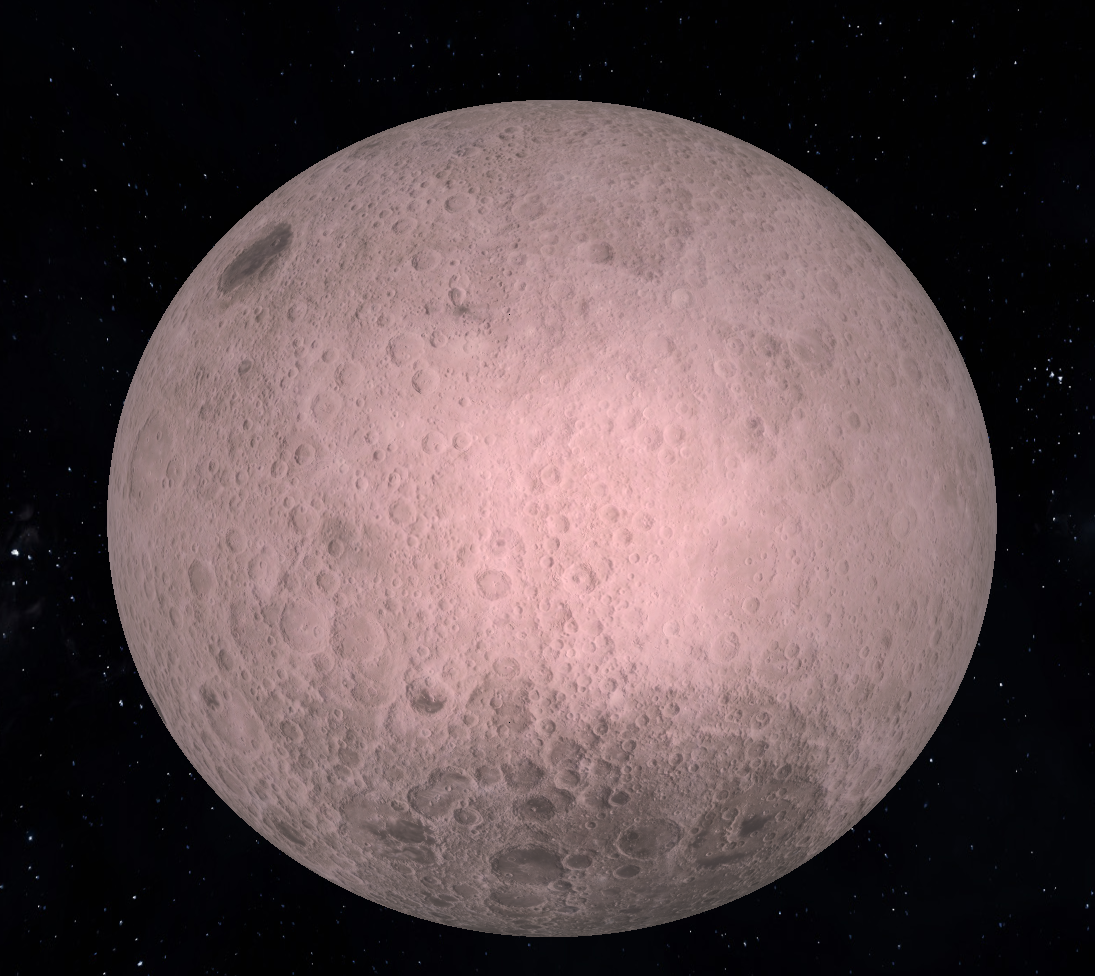
\includegraphics[scale=0.2]{result/moon.png}
\end{center}

\clearpage

Figure below shows the binary stars which were added using buttons for addition of stars. Velocity and position of these newly added stars or planets or moons are calculated on the basis of Newton's law of gravitation.

\begin{center}
	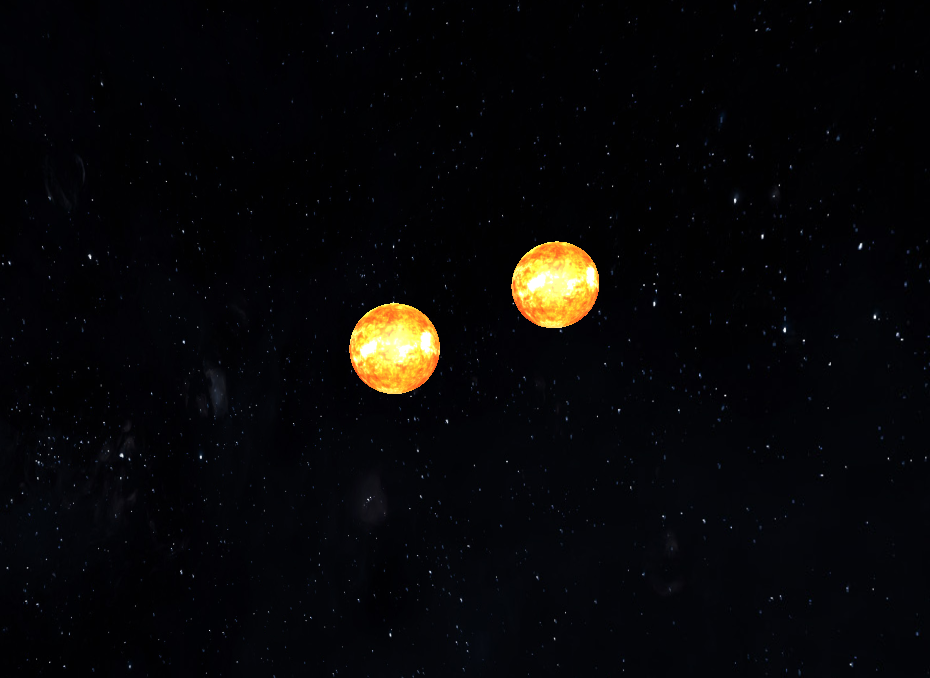
\includegraphics[scale=0.2]{result/bin.png}
	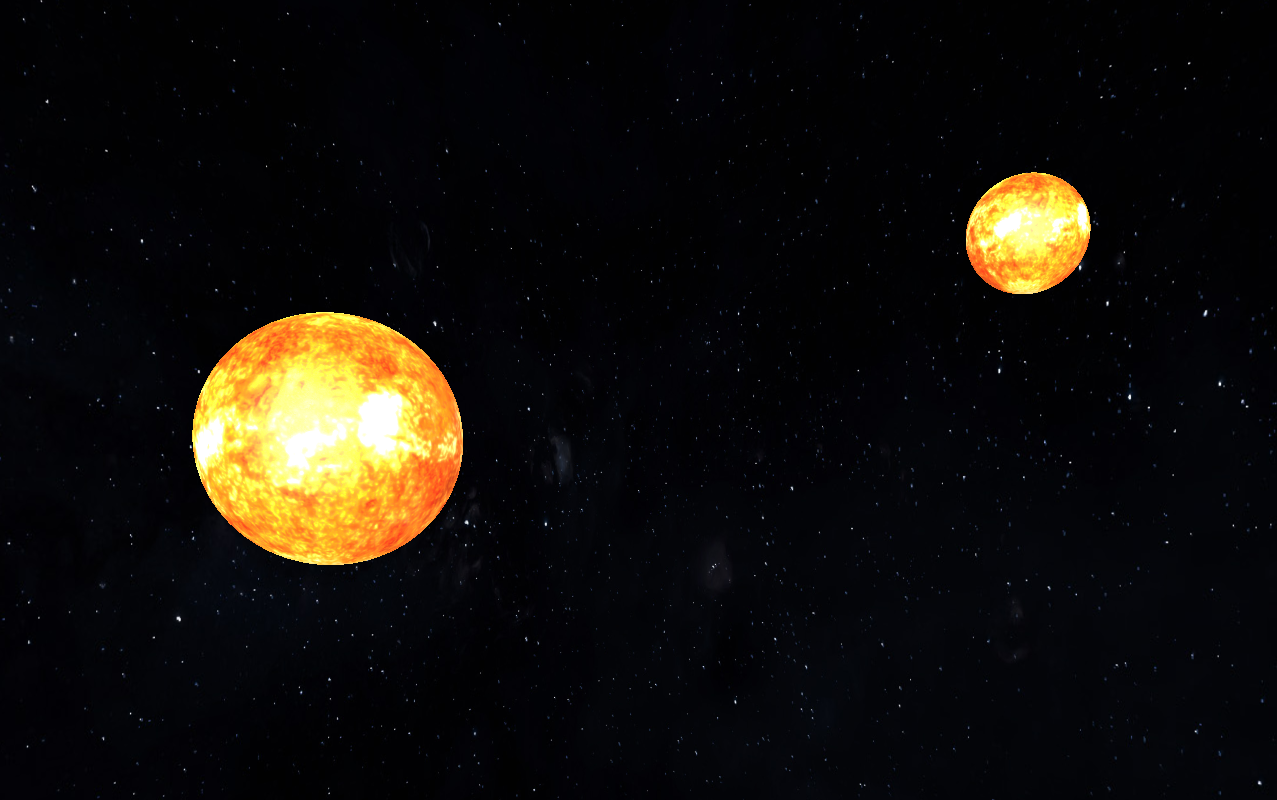
\includegraphics[scale=0.2]{result/bin1.png}
\end{center}


Figure below shows the rendering of solar system. This picture was taken from the mid-term project and it clearly shows the effect of Phong Lighting model.

\begin{center}
	\includegraphics[scale = 0.8]{result/5.png}
\end{center}

\clearpage

\section{Comparision between Mid term project and Final Project}
In mid term project, there was implementation of skybox and sphere development algorithm in order to simulate the solar system. Along with these, Giroud and Phong Lighting model was implemented. All these algorithms were implemented from scratch and the result can be observed below:

\begin{center}
\includegraphics[scale = 0.7]{result/5.png}
\end{center}

Improvements in final project:
\begin{enumerate}
	\item Mathematical modelling of gravity was done using Newton's law of gravitation.
	\item Normal mapping was implemented to enhance the surface details of heavenly bodies.
	\item Matrix stack was used in order to calculate the path of moon.
	\item Addition of heavenly bodies like stars, planets and moons were possible for gravity simulation.
	\item 3D modelling of spacecraft and satellites were created in blender and loaded with OpenGL.
\end{enumerate}

All the changes and improvements can be observed in the result section.

\clearpage
\section{Conclusion}
With the successful implementation of various graphics algorithms and OpenGL C++, Gravity Simulation Project was successfully created. Surface rendering was improved with the use of normal mapping of texture image which was created using GNU image manipulation program(GIMP). Skybox and cube texture coordinates were used so as to create a convincing horizon. Matrix stack was used to calculate the position of the planets. The demo was completed by building solar system and manual addition of planets, stars and moon. 3D modelling of Satellites and Starship was added in the project as a part of 3D model rendering.

\section{Further Enhancement}
\begin{enumerate}
	\item Different other factors like density, axial tilt, composition, etc.  can be added to simulate the rotation and revolution of heavenly bodies. 
	\item Variable size heavenly bodies addition button can be created
	\item Shadow can be added so that we can even observe eclipse.
\end{enumerate}

\section{References}
\begin{itemize}
	\item Gordon,V.Scott and Clevenger,John : Computer Graphics Programming in OpenGL with C++,2021
	\item De Vries, Joey : Learn OpenGL - Graphics programming
	\item Huges, John and Van Dam, Andries : Computer Graphics principles and practices
	\item Baker : Computer Graphics with Open GL
\end{itemize}


\end{document}